\chapter{Sistemas Colaborativos}
\label{capitulodos}

El trabajo en grupo es una actividad humana fundamental y los entornos colaborativos facilitan este proceso. Un aspecto crucial para su estudio y dise\~no es el uso de t'ecnicas eficientes que permitan representar los procesos de comunicaci'on, coordinaci'on y acceso a la informaci'on. Desde el nacimiento de los sistemas computacionales, el trabajo en muchos 'ambitos fue transformado dr'asticamente, con dicho cambio tambi'en surgi'o la necesidad de compartir informaci'on, recursos, memoria y otros.

\medskip
Con la aparici'on de las redes y el internet, se logr'o compartir informaci'on y algunos recursos. Pero a'un no es suficiente, puesto que tambi'en surge la necesidad del trabajo conjunto o en equipo, un claro ejemplo de dichas necesidades es el conocido caso de Linux, un sistema operativo desarrollado por gran cantidad de personas de distintas partes del mundo.
 
\medskip
Debido a la naturaleza de algunas actividades dentro el desarrollo de software, a veces es indispensable incorporar a distintos grupos de personas al momento de desarrollar alg�n trabajo espec'ifico. Dentro del dise\~no de interfaces se recomienda la incorporaci'on de diversos grupos de usuarios como ser: programadores, clientes (alg'un usuario al que va destinado el sistema), dise\~nadores gr'aficos y alg'un otro tipo de usuario que podr�a realizar aportes significativos para el dise\~no. 

\medskip
Lo descrito anteriormente denota un trabajo de colaboraci'on entre distintos tipos de personas con ideas diferentes, pero con un objetivo en com'un. Para coadyuvar en la actividad de dicho grupo, se plantea el uso de un sistema colaborativo.

\medskip
Dado que el foco del proyecto es desarrollar un sistema colaborativo, con el objetivo de identificar la utilidad del mismo dentro del proceso de creaci'on de una interfaz de usuario, es necesario plantear algunos conceptos b'asicos que  servir'an como marco conceptual y de referencia.


\section{CSCW y Sistemas Colaborativos}
Seg'un \cite{garrido2000designing} ``CSCW es una disciplina emergente que analiza el trabajo en grupo asistido por computadora, con una estrecha aplicaci'on en el control de organizaciones y distribuci'on del trabajo''. Sin embargo, este aspecto cada vez tiene un sentido m'as amplio, lo que permite recoger entornos en los cuales se produce interacci'on entre participantes con diversos fines (educativos, visitas tur'isticas, ocio, etc.), con diferentes habilidades de los usuarios implicados, distintos medios y soportes de acceso (computaci'on ubicua). 
El t'ermino ``Computer-supported Cooperative Work (CSCW)'' introducido por Irene Greif y Paul M.Cashman
\cite{brown1985interfaces} se refiere a ``C'omo las actividades colaborativas y su coordinaci'on pueden ser apoyadas por medio de sistemas computacionales.'', CSCW suele ser interpretado como un sin'onimo de sistema colaborativo, sin embargo algunos autores afirman que, mientras los sistemas colaborativos se refieren a sistemas computacionales reales, CSCW se enfoca en estudiar las herramientas y las t'ecnicas de un sistema colaborativo as'i como su impacto psicol'ogico, social y el efecto organizacional que causa. Wilson \cite{wilson1991computer} define los CSCW de la siguiente manera:

\medskip
\emph{``CSCW es un t'ermino gen'erico, que combina la comprensi'on de la forma en que las personas trabajan en grupo usando tecnolog'ias de redes de computadoras y hardware asociado, software, servicios y t'ecnicas.''}
\medskip

En cambio define los Sistemas colaborativos  como:

\medskip	
	\emph{``Actividades de grupo intencionales con software para su apoyo.''}
\medskip	

Dentro del software colaborativo se puede encontrar: los Groupware y Workflow que son las tecnolog'ias m'as usadas y que ser'an brevemente descritas a continuaci'on.

\subsection{Groupware}
La relaci'on usuario m'aquina comenz'o a cambiar a medida que el software fue evolucionando, un claro ejemplo se present'o en software orientado al entretenimiento (videojuegos), que a medida que los usuarios comenzaron a necesitar algo m'as que un mero pasatiempo, se comenz'o a desarrollar caracter'isticas importantes como el soporte a multijugador en l'inea, el cual permite a varios usuarios encontrarse en el mismo videojuego. En muchas labores dentro del 'ambito empresarial se necesita interactuar con grupos de personas, en este contexto trasladar la caracter'istica de esos videojuegos antes mencionada puede ser muy 'util, el interactuar con las personas que necesitas en tiempo real sin necesidad de tenerlos en el mismo lugar geogr'afico, lo cual  representa una gran ventaja al momento de realizar ciertas actividades.
 
 \medskip
Los groupware \cite{ellis1991groupware} son un tipo de sistemas colaborativos que se enfocan en ayudar a los equipos de trabajo a realizar actividades mediante una red. Para describir un Groupware tomaremos la siguiente definici'on:

\medskip 
\emph{``Sistemas basados en computadoras que apoyan a grupos de personas que trabajan en una tarea com'un y que proveen una interfaz para un ambiente compartido'' -Dave Chaffney }
\medskip

Los Groupware hacen 'enfasis en tres caracter'isticas muy importantes: ``Colaboraci'on, Comunicaci'on y Coordinaci'on''  \cite{ellis1991groupware}. Estos tres elementos son fundamentales a la hora de trabajar en equipo. A su vez buscan promover un ambiente compartido de colaboraci'on, en el que se perciba realmente el trabajo en equipo, un ambiente en el que se pueda interactuar con las dem'as personas no solo en el trabajo desempe\~nado, sino tambi'en mediante texto, voz o video.

\medskip
Se puede notar en la definici'on de Groupware que esta no define que el trabajo deba que ser simult'aneo. Estos sistemas pueden proveer diferentes tipos de soporte de acuerdo a las necesidades que se presenten; Si el trabajo dentro del Groupware es efectuado por los usuarios al mismo tiempo, se lo define como s'incrono, de lo contrario, si el trabajo es efectuado en distintos lapsos de tiempo por los usuarios, es definido como as'incrono. Si el trabajo se realiza desde diferentes lugares geogr'aficos se denomina distribuido; esto puede verse de mejor manera en la siguiente figura \ref{fig:GroupWareTimeMatrix}:

\begin{figure}[ht]
\centering
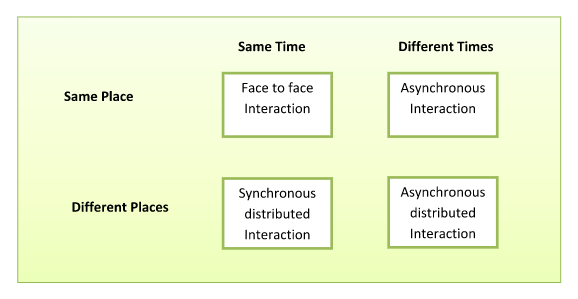
\includegraphics[width=0.75\textwidth]{Figura0201GroupWareTimeMatrix}
\caption{Groupware Time Space Matrix. Fuente:}
\cite{ellis1991groupware}
\label{fig:GroupWareTimeMatrix}
\end{figure}
\medskip

CSCW se convirti'o en un campo de investigaci'on amplio que abarca desde el an'alisis sociol'ogico sobre la forma de trabajar en grupos a las tecnolog'ias inform'aticas que apoyan el trabajo en grupo de las personas. 

\medskip
Existe una delgada l'inea que separa a los sistemas que son considerados groupware y los que no. El criterio m'as importante \cite{ellis1991groupware} para poder definir un groupware es el soporte que ofrece al trabajo en equipo, por ejemplo un sistema que brinda soporte al trabajo de m'ultiples usuarios, pero en 'areas diferentes y realizando tareas diferentes tiene un bajo nivel de cooperaci'on, a diferencia de un sistema pensado para dar soporte a m'ultiples usuarios realizando una tarea conjunta en un espacio compartido, por ejemplo el caso de google docs.
El desarrollo de software es una actividad donde el trabajar de manera distribuida es algo que sucede regularmente, se tienen varios ejemplos grandes de dicha situaci'on como ser el conocido caso del sistema operativo Linux.

\medskip
Entre los criterios que se toman para catalogar un groupware como tal, est'an el desarrollar la misma tarea y el estar presentes en espacio compartido. Por ejemplo, un sistema de tiempo compartido permite que m'ultiples usuarios realicen actividades, pero estos pueden tener metas diferentes, por lo tanto realizar'an tareas diferentes, en cambio un sistema que permite editar un documento de manera conjunta (google docs), est'a enfocado a que los usuarios que ingresen al sistema tengan en mente una misma meta, lo cual se refleja en las actividades que se realicen. De igual forma un sistema de mensajer'ia permite que dos usuarios puedan interactuar y enfocarse en una misma tarea, pero el ambiente y la colaboraci'on no son muy notorios, en cambio el sistema que permite el dise\~no de la interface tiene que dar soporte para que los usuarios puedan percibir lo que sus compa\~neros est'an haciendo.

\subsection{Workflow}

\medskip
Los Workflows son sistemas que ayudan a administrar y automatizar procesos de negocios en los que participan diferentes usuarios.

La WfMC (Workflow Management Coalition) define a los Workflows Como:

\medskip 
\emph{``La automatizaci'on de un proceso de negocio, total o parcial, en la cual documentos, informaci'on o tareas son pasadas de un participante a otro a los efectos de su procesamiento, de acuerdo a un conjunto de reglas establecidas.''}
\medskip

En la misma definici'on radica la diferencia entre groupware y workflow, dado que los groupware son sistemas orientados al trabajo conjunto, en cambio los workflow est'an orientados dar soporte al conjunto de personas que realizan distintas tareas siguiendo un flujo de trabajo. Debido a los diferentes tipos de procesos que se pueden dar soporte con un workflow se definen:

\medskip 
a) Workflows de Producci'on: o tambi'en llamados Workflows de transacciones; las transacciones son la base de las acciones dentro de las bases de datos, los workflow de producci'on en general automatizan procesos de negocios que tienden a ser repetitivos y con gran manejo de datos.

\medskip
b) Workflows de Colaboraci'on: Los workflow que est'an orientados a resolver procesos de negocios donde participan grupos de personas que tienen una meta com'un son denominados Workflows de colaboraci'on.

\medskip
c) Workflows de Administraci'on: Son aquellos que est'an orientados a dar soporte a la los procesos de administraci'on de una empresa o negocio.
\medskip

Se puede afirmar que los Workflow son herramientas muy 'utiles para identificar y evaluar procesos, tambi'en son muy importantes al hacer un trabajo de reingenier'ia puesto que su principal enfoque es el integrar a las personas y los procesos que se llevan a cabo dentro de un negocio.

\medskip
Despu'es de haber definido la diferencia entre groupware and workflow y tomando en cuenta las caracter'isticas que ambas opciones presentan, se opt'o por los Groupware como el centro te'orico del presente proyecto, dadas las facilidades en el apoyo a la colaboraci'on dentro de un trabajo grupal, que es exactamente lo que se busca al momento de dise\~nar interfaces de usuario.


\section{Awareness}
En un WYSIWIS (What you see is what I see- Lo que ves es lo que veo) relajado, los usuarios pueden trabajar en diferentes partes de un espacio compartido. En dicha circunstancia es importante que el usuario sea consciente del estado de los otros usuarios, para que de esa manera pueda colaborar de manera natural y fluida con ellos. En este 'ambito se habla de la conciencia de grupo (awareness) tambi'en definida como momento de comprensi'on de la interacci'on de otra persona con el espacio compartido. \cite{gutwin1996workspace}

\medskip
El awareness es fundamental en los sistemas colaborativos, puesto que incrementa significativamente la usabilidad del sistema \cite{gutwin1996workspace}. Es usado principalmente para, simplificar la comunicaci'on, coordinar acciones, ayudar a los usuarios a anticipar futuras acciones y entender la ayuda de los dem'as. \cite{gutwin1996workspace}, la informaci'on de la conciencia de grupo consiste en los diferentes elementos listados en la siguiente figura \ref{fig:WorkspaceAwareness}.

\begin{figure}[ht]
    \centering
    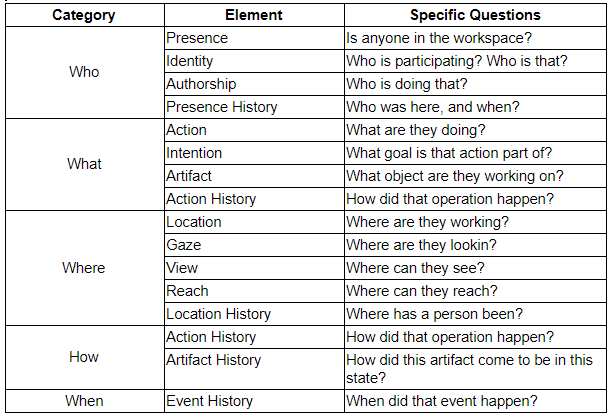
\includegraphics[width=0.75\textwidth]{Figura0202WorkspaceAwareness}
    \caption{Composition of workspace awareness information. Fuente: Grudin and Greenberg 2002}
    \label{fig:WorkspaceAwareness}
\end{figure}
\medskip

La primera columna de la tabla lista b'asicamente las categor'ias de la informaci'on del awareness, incluyendo: con quien estamos trabajando, que es lo que est'an haciendo, donde estan, como estan ocurriendo dichos eventos, cuando estos eventos est'an sucediendo. 

\medskip
En cada categor'ia existen diferentes elementos de conciencia, cada elemento describe una respuesta a cada pregunta que se puede realizar dentro de un espacio compartido las cuales se muestran en la tercera columna. (Gutwin and Greenberg 2002). 

\medskip
Para llenar la informaci'on requerida en el awareness, existen diferentes herramientas que son usadas com�nmente por los sistemas colaborativos:

\medskip
Telepointer: El telepointer es la manifestaci'on del puntero remoto de otro usuario, que se muestra en el sistema del usuario local.

\medskip
Multi-user Scrollbar: el multi-user scrollbar es una extensi'on del scrollbar simple, que indica la posici'on de los dem'as usuarios.

\medskip
Radar view: el radar view es una herramienta para entregar una informaci�n m'as detallada de la ubicaci'on de un usuario, se usa generalmente cuando el sistema colaborativo presenta m'as de un espacio compartido para el trabajo.

\medskip
En adici'on a las herramientas descritas existen otras no tan frecuentes que pueden ser de gran ayuda de acuerdo a las caracter�sticas del sistema en cuesti'on, dichas herramientas pueden ser el sonido, una lista de usuarios con la informaci'on de su sesi'on, video, areas de intercambio de mensajes, entre otros.


\section{AMENITIES: Metodolog'ia para el estudio y desarrollo de sistemas cooperativos}
Cuando se realiza alg'un proceso que implica la colaboraci'on entre personas, lo primero que se debe tener en cuenta es la estructura y la organizaci�n de dicho grupo de trabajo. Como resultado se tienen como tareas fundamentales el recoger los aspectos organizativos, cognitivos y de interacci�n que representen de manera adecuada las demandas del trabajo en concreto.

Existen propuestas dentro del dise\~no de sistemas colaborativos que ofrecen notaciones con diferente nivel de formalismo y abstracci'on para recoger aspectos relativos a dichos sistemas. Dentro de la amplia gama de propuestas se encuentran GTA [welie] y ConcurTaskTrees [Paterno,97]. La primera se centra en la descomposici'on de tareas y asignaci�n de actividades a roles, en cambio CTT se centra m'as en aspectos de coordinaci'an ( uso temporal de espacios comunes), sin embargo estas propuestas no dejan de ser parciales y no cubren las caracter�sticas de los sistemas colaborativos, a su vez son dif'iciles de enlazar con tecnicas de Ingenieria de Software.

Para trabajar sobre la complejidad inherente a los entornos colaborativos, se ha propuesto el uso de una metodolog'ia conocida como ``AMENITIES'', que permite describir un sistema colaborativo mediante cuatro vistas que facilitan detectar los aspectos m'as relevantes de los sistemas de este tipo.

AMENITIES (acr'onimo de A Methodology for aNalysis and DesIgn of CooperaTIve systEmS) [Garrido, 03] integra de modo jerarquizado varios modelos de comportamiento y tareas, con la idea de proporcionar una representaci'on del sistema colaborativos en su conjunto y con diferentes vistas complementarias. 


\subsection{Vista de grupo}

Para la vista de grupo, primeramente se debe identificar los aspectos propios del grupo u organizaci'on, y las restricciones que se imponen. Dichas organizaciones se articulan bajo ``roles'', que determinan las relaciones entre los miembros del grupo y las tareas que est'an bajo su cargo. 

Las relaciones, normalmente est'an condicionadas por una serie de restricciones impuestas al sistema colaborativo, y se pueden identificar como m'as importantes las siguientes:

\begin{itemize}
	\item Capacidades: Son restricciones cognitivas que se imponen a cada actor para participar en un rol determinado. Estas capacidades determinan los conocimientos que se debe adquirir por un usuario para participar en un rol concreto.
    \item Leyes: Son restricciones impuestas por la organizaci'on e identifica las reglas que se deben preservar en un grupo. Normalmente estas reglas son la misma estructura social que se manifiesta en el grupo(jerarqu'ia, democracia, etc.)
\end{itemize}

Ambas restricciones permiten modelar sistemas din'amicos, es habitual que tanto la estructura del grupo como su funcionamiento se modifique en el tiempo (los participantes pueden adquirir nuevas capacidades, variar en n'umero de miembros que lo conforman o bien, modificar las leyes que rigen el grupo al aplicar nuevas estrategias de trabajo). 


\subsection{Vista de cognitiva}
La vista cognitiva representa el conocimiento que posee o adquiere cada miembro del grupo en el escenario colaborativo. Este conocimiento queda reflejado mediante la descripci'on de las tareas que puede llevar a cabo.

La descripci'on de las tareas implica un an'alisis profundo de las actividades que se deben realizar en el grupo, la divisi'on del trabajo y determinar las interrelaciones que existen entre ellas. El an'alisis de tareas contempla todos estos pasos, y las divide en dos fases claramente diferenciadas. 

En primer lugar se define la denominada interfaz del rol, que recoge las caracter'isticas m'as relevantes de las tareas a desempe\~nar por un rol junto a las interrelaciones con el resto de participantes (tareas) y entorno (mediante eventos).
 
Los aspectos m'as relevantes que identificamos en el interfaz del rol son:

\begin{itemize}
	\item Identificar tareas a desempe\~nar
	\item Relaci'on con otras tareas tales como:
	\begin{itemize} 
		\item Si puede ser interrumpida por otra tarea 
		\item Su naturaleza cooperativa 
		\item Mecanismo de activaci'on y modos de sincronizaci'on 
	\end{itemize}
\end{itemize}

\medskip

Este tipo de relaciones modelan el comportamiento tanto del usuario como del propio entorno. Las mismas se modelan mediante eventos que provocan cambios en el entorno (y en las pol'iticas que determinan el comportamiento del sistema). 

\medskip

En la segunda fase, se describe y pormenoriza cada tarea mediante una descomposici'on jer'arquica, que se completa con informaci'on y aspectos recogidos de otras vistas. En esta descripci'on de tareas usaremos notaciones que nos permite especificar secuencialidad, concurrencia, optatividad, decisiones, etc.

\medskip
Posteriormente, se detalla las tareas tanto individuales como cooperativas, y en las cuales, puede aparece informaci�n relativa a otras vistas.

\subsection{Vista de interacci'on}
La vista de interacci�n abarca otros aspectos que se deben estudiar como ser los procesos que implican un di�logo entre participantes para analizar sus caracter�sticas, concretamente: 

\begin{itemize}
	\item El modo de di�logo que se producen entre participantes 
	\item Los requisitos que impone ese di�logo sobre los medios a utilizar
\end{itemize}

\medskip
Este modo de di�logo se identifica mediante protocolos. Los protocolos se pueden analizar por separado dentro de la organizaci�n ya que en gran medida son independientes del dominio del problema, y por tanto, se pueden incorporar al an�lisis de tareas. Por ejemplo, se pueden identificar protocolos democr�ticos (toma de una decisi�n por mayor�a), consenso (aprobaci�n un�nime de una decisi�n), jer�rquica, etc.

\subsection{Vista de informaci'on}

En la vista de informaci'on, se debe recoger la informaci'on que es compartida en el escenario. Esta informaci'on se puede describir de manera impl'icita en las actividades y acciones o bien, de modo expl'icito como flujo de informaci'on entre actividades. La informaci'on que fluye a trav'es del sistema colaborativo ser'an los documentos (los objetos que son gestionados en el sistema), eventos y recursos. 

\section{Refactorizaci'on}

AMENITIES est'a centrada en el modelado inicial del sistema usando el punto de vista del usuario y teniendo muy en cuenta aspectos relacionados con el grupo (conciencia de grupo, relaciones entre usuarios, din'amica del grupo, representaci'on de aspectos sociales, etc), dicha definici'on permite la posibilidad del desarrollo de un sistema colaborativo ya sea desde su inicio, o transform'andolo a partir de un sistema ya realizado, agregando las caracter'isticas ya mencionadas, puesto que la din'amica de grupo representa la evoluci'on del contexto en el que se va a realizar la colaboraci'on entre los usuarios.

\medskip
Durante el desarrollo de sistemas colaborativos, existen dos opciones, la creaci'on de un sistema colaborativo o refactorizar una aplicaci'on mono-usuario en una aplicaci'on multi-usuario [Qian Xia, 06], para realizar la refactorizaci'on se debe tomar en cuenta los siguientes requerimientos:

\begin{itemize}
	\item Compatibilidad de la Aplicaci'on: Las caracter'isticas de la interfaz, funcionalidades y formatos de la aplicaci'on mono-usuario original deben mantenerse.

	\item Transparencia de la aplicaci'on: no deben realizarse cambios en el c'odigo fuente original.

	\item Respuesta local r'apida: la interacci�n con el sistema en un medio local debe ser tan r'apida como la respuesta del sistema original.

	\item Colaboraci'on sin restricci'on: Se debe permitir a los usuarios cualquier operaci'on sobre objetos de datos en cualquier momento, lo que implica un WYSIWIS (What you see is what i see) relajado y trabajo simultaneo.
	\item Workspace Awareness: El sistema debe soportar una variedad de caracter'isticas relacionadas a la conciencia de grupo dentro de los espacios de trabajo, de tal manera el usuario puede saber quien esta en su grupo de trabajo, donde se est'a trabajando y que es lo que se est'a trabajando.

	\item Administraci'on de sesi'on: El sistema debe proveer una administraci'on de sesi'on ligera y flexible, para soportar que usuarios administran el trabajo con poco esfuerzo.

	\item Control de interacci'on flexible: El sistema debe proporcionar una variedad de control de interacci'on paradigmas / pol'iticas que van desde la interacci'on simult'anea y libre, hasta la interacci'on secuencial y sincronizada con el fin de facilitar la eficacia de diferentes tareas de colaboraci'on.

\end{itemize}

\medskip
Debido a que la refactorizaci'on de un sistema puede llegar a tornarse bastante compleja, existen trabajos previos que sirven como marco de referencia para futuros trabajos, tal es el caso de CoWord y CoPowerPoint aplicaciones colaborativas realizadas a partir de Word y PowerPoint respectivamente [Qian Xia, 06].

\subsection{Arquitectura centralizada y replicada}

Al momento de realizar un sistema colaborativo, se debe escoger la arquitectura que soporta la aplicaci�n, la arquitectura de los sistemas colaborativos puede ser clasificada en dos grupos, la arquitectura centralizada y la arquitectura replicada (Lauwers, 90).

\medskip
Con la arquitectura centralizada, existe 'unicamente una instancia de la aplicaci'on compartida ubicada en un sitio central. Los dem'as sitios colaborativos cuentan simplemente con sistemas clientes que cuentan con funciones limitadas de acuerdo al rol que desempe\~nan dentro del plan de trabajo. El cliente b'asicamente dispara eventos para la aplicaci�n compartida, dichos eventos generan informaci'on en el sistema central de la aplicaci'on, la cual luego es distribuida y mostrada en el o los sistemas cliente.

\begin{figure}[ht]
    \centering
    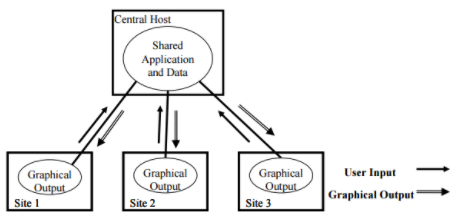
\includegraphics[width=0.75\textwidth]{Figura0203ArquitecturaCentralizada}
    \caption{Arquitectura centralizada. Fuente: Lauwers 90 }
    \label{fig:ArquitecturaCentralizada}
\end{figure}
\medskip

La principal ventaja de la arquitectura centralizada es su facilidad de implementaci'on a comparaci'on de la arquitectura replicada puesto que solamente se tiene que mantener una instancia de la aplicaci'on compartida, los desarrolladores no tienen que poner mucha energ'ia en la consistencia de la informaci'on. Pero la centralizaci�n tambi'en presenta desventajas, la m'as significativa es la lentitud en la respuesta local, cada evento local debe ser enviado a la aplicaci'on compartida, la vista local no puede ser actualizada hasta que la informaci'on sea recibida correctamente en la aplicaci'on central. La espera puede tornarse muy alta mientras mayor sea el retardo de la red. 

\medskip
Dichos problemas motivaron la arquitectura replicada, en la que cada uno de los sitios colaboradores tiene una instancia de la aplicaci'on compartida, corriendo en el sitio local. La arquitectura replicada es capaz de realizar una respuesta r'apida gracias a que los eventos disparados por el usuario pueden ser ejecutados de manera local antes de ser enviados a los sitios remotos. 

\begin{figure}[ht]
    \centering
    \includegraphics[width=0.75\textwidth]{Figura0204ArquitecturaReplicada}
    \caption{Arquitectura replicada. Fuente: Lauwers 90 }
    \label{fig:ArquitecturaReplicada}
\end{figure}
\medskip

De cualquier manera la arquitectura replicada tambi'en presenta problemas, el m'as significativo es mantener la consistencia. Si se permite a los usuarios interactuar con su aplicaci'on local y replicar libremente, los eventos pueden ser ejecutados en diferente orden en los distintos sitios distribuidos. Sin embargo la arquitectura replicada facilita el WYSIWIS y tambi'en elimina el retardo en el tiempo de respuesta de la aplicaci'on.


%(8-10pp)